\section{Unitary Transforms}

Images can be either written as matrices or as vectors to make math easier. So a linear image processing system can be defined as:
$$g = \textbf A f$$

So we ask ourself the question how to choose $\textbf A$. We say $\textbf A$ is unitary (or orthonormal for real values) if $\textbf A^{-1} = \textbf A^H$. Transformations by unitary matrices are energy conserving, meaning the length of the transformed vector will stay the same.

We introduce the following notation: $f_i$ one image, $F = [f_1, ..., f_n]$ collection of images and $R_{ff} = E[f_i \cdot f_i^H] = \frac{F \cdot F^H}{n}$ image collection auto-correlation function. While unitary transformations preserve the energy, it will often be unevenly distributed among coefficients. The autocorrelation matrix of the transformed image will look like this: 
$$R_{cc} = \textbf A R_{ff} \textbf A^H$$

The eigenmatrix $\Phi$ of $R_{ff}$ is unitary and defined as follows:
\begin{center}
	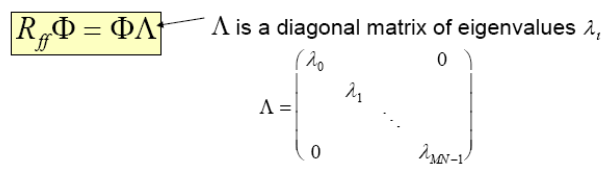
\includegraphics[width=\linewidth]{eigenmatrix.png}
\end{center}

\subsection{Karhunen-Loeve Transform / PCA}

If we choose $\textbf A = \Phi^H$ we get:
$$R_{cc} = \Phi^H R_{ff} \Phi = \Phi^H \Phi \Lambda = \Lambda$$

We can interpret this transformation as follows: "No other unitary transformation packs as much energy into the first $k$ coefficients, where $k$ is arbitrary". The mean squared approximation error by choosing only the first $k$ coefficients is minimized. 
\begin{center}
	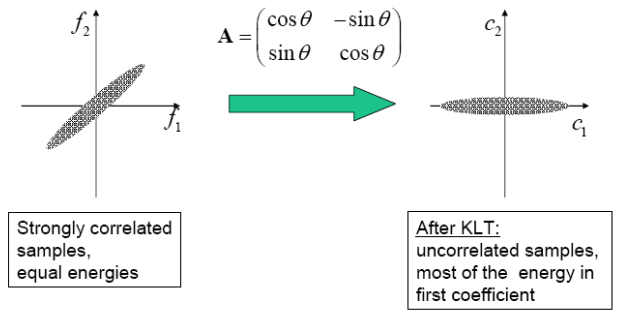
\includegraphics[width=\linewidth]{energy_concentration.png}
\end{center}

The basis images, which are the eigenvectors of the autocorrelation matrix, are called \textbf{eigenimages}. We can use eigenimages for recognition tasks, as the high dimensionality of the images space can be reduced to $k$ dimensions. To perform recogintion, we tailor a KLT / PCA to the specific set of images we want to recognize, for example this lead to Eigenfaces. \medskip

The first principal component is the eigenvector with the largest eigenvalue. The eigenvalue can be interpreted as denoting the variance in the direction of the corresponding eigenvector. So the principal component shows in which direction the data is most spread out.

\subsubsection{Fisherfaces}

To improve on the short comings of Eigenfaces, Fisherfaces try to find the direction where the ratio between individual variance are maximized. As the math behind this is rather complex, it is left out.
\begin{center}
	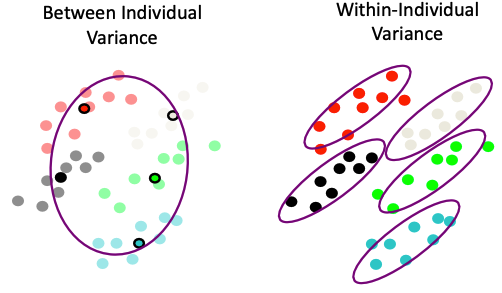
\includegraphics[width=0.8\linewidth]{fisher.png}
\end{center}


\subsection{JPEG Compression}

We notice that humans do not resolve high frequencies too well, therefore we can leave some of them away to reduce the size of an image.
\begin{center}
	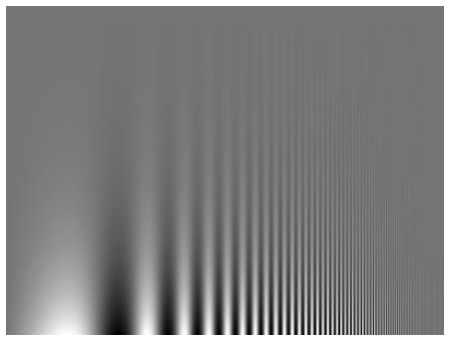
\includegraphics[width=0.8\linewidth]{campbell_robson.png}
\end{center}

This is one of the main concepts in JPEG compression. Instead of FT, JPEG uses discrete cosine transform (DCT), which has no imaginary part. We go through the components of the DCT in a snake like pattern.
\begin{center}
	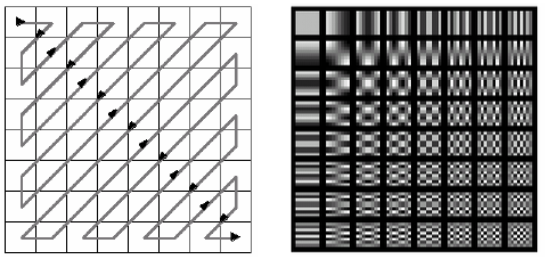
\includegraphics[width=\linewidth]{jpeg_compression.png}
\end{center}

If the coefficients get too small after a certain point, we simply leave them away. In the end we apply Huffman encoding to further reduce the size of our image. \medskip

JPEG tends to introduce three kinds of distortions:
\begin{itemize}
	\item General loss of sharpness and oscillations around high-contrast edges: these are due to approximating intensity transitions with smooth functions (cosines).
	\item Blocking structure: image is processed separately for every 8x8 block, block edges become visible at high compression ratios.
	\item Loss of color detail: the program may aggressively "downsample" chromaticity channels.
\end{itemize}
